\documentclass[10pt]{article}
\usepackage{geometry}                % See geometry.pdf to learn the layout options. There are lots.
\usepackage{blindtext}
\usepackage[parfill]{parskip}    % Activate to begin paragraphs with an empty line rather than an indent
\usepackage{tikz}
\usetikzlibrary{arrows,automata,shadows,positioning,shapes}
\usepackage{graphicx}
\usepackage{amssymb}
\usepackage{amsmath}
\usepackage{amsthm}
\usepackage{epstopdf}
\usepackage{hyperref}
\usepackage{listings}
\usepackage{subfiles}
\usepackage[utf8]{inputenc}
\usepackage{float}
\usepackage{tikz}
\usepackage{graphicx}
\usepackage{caption}
\usepackage{wrapfig}


\newcommand{\NEXP}{\textsf{NEXP}}
\newcommand{\EXP}{\textsf{EXP}}
\newcommand{\EPE}{\textsf{$E=P^{E}$}}
\newcommand{\PH}{\textsf{PH}}
\newcommand{\PS}{\textsf{PSPACE=NPSPACE=AP=IP}}
\newcommand{\BPP}{\textsf{BPP}}
\newcommand{\PPoly}{\textsf{$P_{/poly}$}}
\newcommand{\NP}{\textsf{NP}}
\newcommand{\coNP}{\textsf{coNP}}
\newcommand{\cP}{\textsf{P}}
\newcommand{\coRP}{\textsf{coRP}}
\newcommand{\RP}{\textsf{RP}}
\newcommand{\ZPP}{\textsf{ZPP}}
\newcommand{\cNL}{\textsf{coNL}}
\newcommand{\NL}{\textsf{NL}}
\newcommand{\cL}{\textsf{L}}

\title{Computational Complexity Theory - Assignment 11}
\author{Alex Hoppen (334784), Jan Uthoff (310336)}

\begin{document}

  \maketitle
  \section*{Exercise 41}

  \begin{figure}[h]
    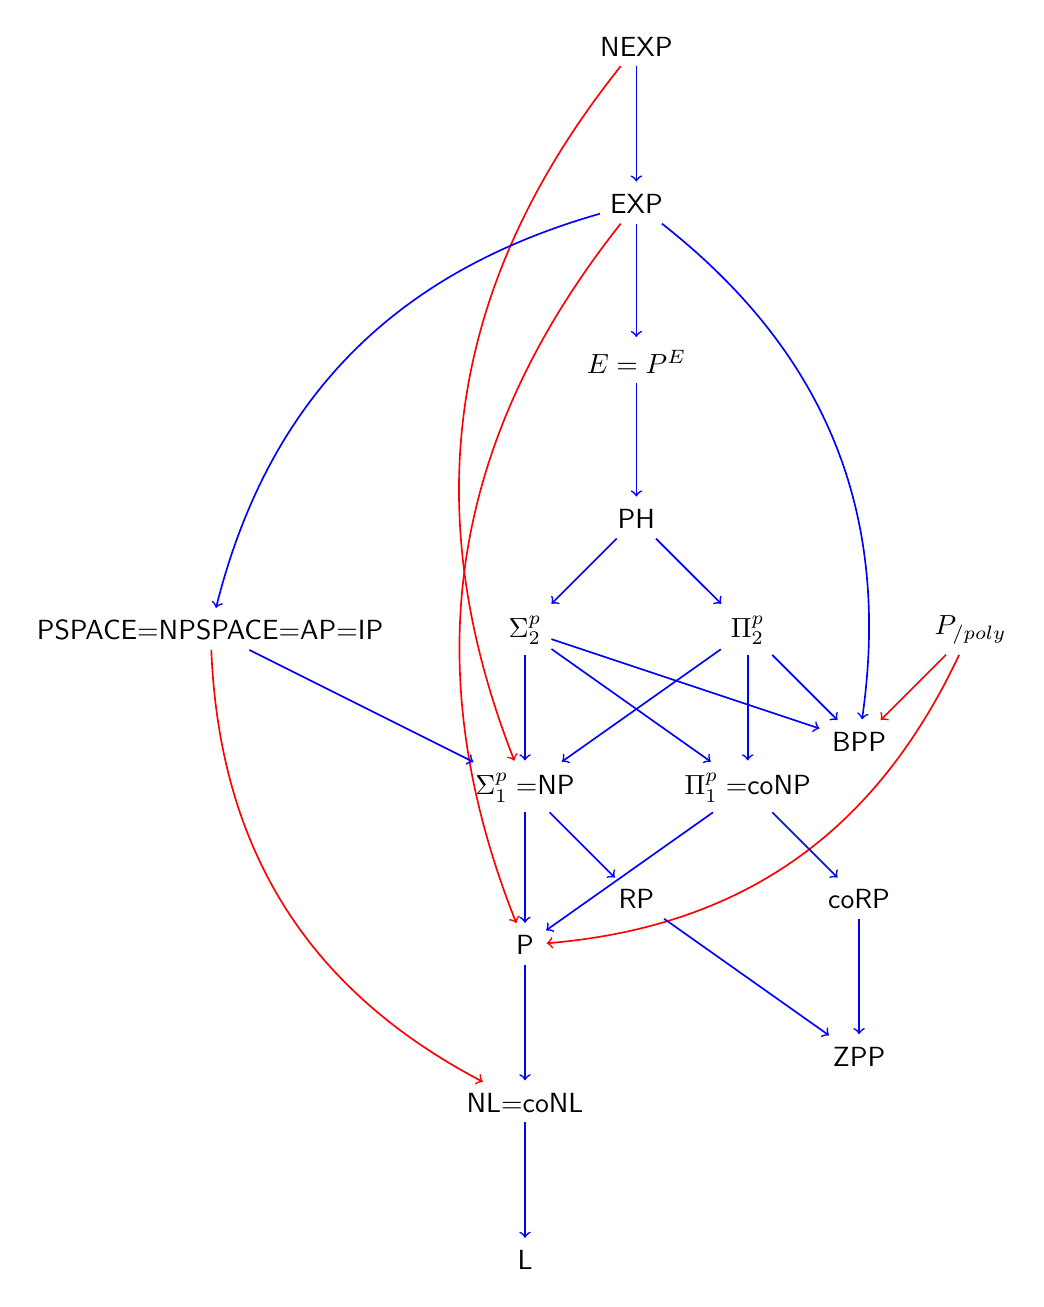
\begin{tikzpicture}[shorten >=1pt,auto,semithick,node distance = 2cm]
      \node (nexp)                              {\NEXP};
      \node (exp) [below of=nexp]               {\EXP};
      \node (epe) [below of=exp]                {\EPE};
      \node (ph)  [below of=epe]                {\PH};
      \node (s2)  [below left of=ph]            {$\Sigma_{2}^{p}$};
      \node (p2)  [below right of=ph]           {$\Pi_{2}^{p}$};
      \node (empty)[left of=s2] {};
      \node (ps)  [left of=empty]               {\PS};
      \node (bpp) [below right of=p2]           {\BPP};
      \node (pp)  [above right of=bpp]          {\PPoly};
      \node (np)  [below of=s2]                 {$\Sigma_{1}^{p}=$\NP};
      \node (cnp) [below of=p2]                 {$\Pi_{1}^{p}=$\coNP};
      \node (crp) [below right of=cnp]          {\coRP};
      \node (rp)  [below right of=np]           {\RP};
      \node (zpp) [below of=crp]                {\ZPP};
      \node (p)   [below of=np]                 {\cP};
      \node (nl)  [below of=p]                  {\NL$=$\cNL};
      \node (l)   [below of=nl]                  {\cL};

      \path[->] (nexp)  edge [bend right, color=red] (np)
                        edge [color=blue]            (exp);
      \path[->] (exp)   edge [bend right, color=red] (p)
                        edge [bend right, color=blue](ps)
                        edge [color=blue]            (epe)
                        edge [bend left, color=blue] (bpp);
      \path[->] (epe)   edge [color=blue]            (ph);
      \path[->] (ph)    edge [color=blue]            (s2) 
                        edge [color=blue]            (p2);
      \path[->] (ps)    edge [bend right, color=red] (nl)
                        edge [color=blue]            (np);
      \path[->] (s2)    edge [color=blue]            (cnp)
                        edge [color=blue]            (bpp)
                        edge [color=blue]            (np);
      \path[->] (p2)    edge [color=blue]            (np)
                        edge [color=blue]            (cnp)
                        edge [color=blue]            (bpp);
      \path[->] (pp)    edge [color=red]             (bpp)
                        edge [bend left, color=red]  (p);
      \path[->] (np)    edge [color=blue]            (rp)
                        edge [color=blue]            (p);
      \path[->] (cnp)   edge [color=blue]            (crp)
                        edge [color=blue]            (p);
      \path[->] (rp)    edge [color=blue]            (zpp);
      \path[->] (crp)   edge [color=blue]            (zpp);
      \path[->] (p)     edge [color=blue]            (nl);
      \path[->] (nl)    edge [color=blue]            (l);
    \end{tikzpicture}

    \caption{Arrow description:\\$\mathcal{L}$\textcolor{blue}{$\rightarrow$}$\mathcal{L}':\mathcal{L}\subseteq
    \mathcal{L}'$ \\
    $\mathcal{L}$\textcolor{red}{$\rightarrow$}$\mathcal{L}':L\subsetneq
    \mathcal{L}'$}
  \end{figure}


\end{document}

